%=====================================================================
%  Proyecto 2 - Arquitectura de Computadoras
%  Arquitecturas paralelas para la multiplicación de matrices en gem5
%  (GEMM en modo SE, ARMv8 + SVE)
%
%  Convención: \pendiente{...} marca texto que falta (sale en rojo en el
%  PDF). Antes de entregar: buscar "pendiente" y que no quede ninguno.
% =====================================================================
\documentclass[journal]{IEEEtran}
\usepackage[utf8]{inputenc}
\usepackage[T1]{fontenc}
\usepackage[spanish,es-tabla,es-nodecimaldot]{babel}
\usepackage{float}
\usepackage{graphicx}
\usepackage[justification=centering]{caption}
\usepackage{amsmath,amssymb}
\usepackage{pgfplots}
\pgfplotsset{compat=1.18}
\usepackage{siunitx}
\sisetup{output-decimal-marker={,}, group-separator={\,}, group-minimum-digits=4,
  per-mode=symbol, range-phrase={~a~}, range-units=single}
\usepackage{xcolor}
\usepackage{listings}
\usepackage[style=ieee, backend=biber]{biblatex}
\addbibresource{referencias.bib}
\renewcommand*{\bibfont}{\footnotesize}
\usepackage{csquotes}
\usepackage{url}
\hyphenation{mul-ti-pro-ce-sa-dor co-he-ren-cia su-per-es-ca-lar
             vec-to-rial pa-ra-le-lis-mo}

\newcommand{\pendiente}[1]{\textcolor{red}{[PENDIENTE: #1]}}

\definecolor{fondo}{rgb}{0.97,0.97,0.97}
\lstdefinestyle{shell}{
  basicstyle=\ttfamily\scriptsize,
  backgroundcolor=\color{fondo},
  frame=single, rulecolor=\color{gray!50},
  breaklines=true, showstringspaces=false, captionpos=b,
  xleftmargin=4pt
}
\lstset{style=shell}

\begin{document}

% ---------------------------------------------------------------------
%  Datos del informe
% ---------------------------------------------------------------------
\newcommand{\titulo}{Arquitecturas Paralelas para la Multiplicación de
  Matrices en gem5}
\newcommand{\curso}{EL4314 Arquitectura de Computadoras}

\renewcommand{\thetable}{\arabic{table}}
\renewcommand{\figurename}{Fig.}
\renewcommand\IEEEkeywordsname{Palabras clave}

\title{\titulo}
\author{Matías Camacho Abarca, jeacamacho@estudiantec.cr \\
Victoria Cerdas López, 	vicerdas@estudiantec.cr \\
Wilbert Román Rodríguez, alonso05rr01@estudiantec.cr\\
Marvin Zelaya Luna, mzelaya@estudiantec.cr}
\maketitle
\markboth{\curso. \titulo}{}

% ---------------------------------------------------------------------
\begin{abstract}
Se evalúa, mediante simulación en gem5 (modo SE, ARMv8 con SVE), qué
combinación de número de núcleos, ancho superescalar, longitud vectorial
y protocolo de coherencia minimiza el tiempo de ejecución de una
multiplicación de matrices densas en precisión simple (GEMM) bajo un
presupuesto de 32 unidades de costo. Se estudian por separado una línea
base de un núcleo (E1), el ancho y la ventana de un núcleo fuera de
orden (E2), la extensión vectorial SVE (E3), un multiprocesador de
memoria compartida (E4) y los protocolos MESI y MOESI ante falso
compartido (E5), y con esos resultados se exploran configuraciones bajo
el presupuesto (E6). Todas las métricas se extraen solo de la región de
interés. En E4, el GEMM paralelizado por filas alcanza un
\textit{speedup} de $7{,}996\times$ con 8 núcleos O3 de ancho 2 para
$N=128$, con una fracción serial estimada por la ley de Amdahl del
orden de $10^{-4}$; al medir el programa completo, la inicialización
serial y la creación de hilos elevan esa fracción a \SI{1,6}{\percent}
y limitan el \textit{speedup} a $7{,}17\times$.
\pendiente{completar con los resultados principales de E1--E3, E5 y la
arquitectura recomendada en E6 (configuración, costo y tiempo).}
\end{abstract}

\begin{IEEEkeywords}
gem5, GEMM, ARMv8, SVE, superescalar, multiprocesador, ley de Amdahl,
coherencia de caché, MESI, MOESI, falso compartido.
\end{IEEEkeywords}

% =====================================================================
\section{Introducción}

La multiplicación de matrices densas $C = A \times B$ es el núcleo
computacional de las capas totalmente conectadas de una red neuronal y
concentra más del \SI{80}{\percent} de su cómputo. Para un procesador de
inferencia en el borde, el área y la energía están acotadas, de modo que
el problema de diseño no es solo acelerar GEMM, sino decidir en qué
recurso invertir un presupuesto limitado: más núcleos, núcleos más
anchos o registros vectoriales más largos.

Este trabajo actúa como el equipo de arquitectura de ese procesador y
responde la pregunta: \emph{con un presupuesto de 32 unidades de costo,
¿qué combinación de núcleos, ancho superescalar, longitud vectorial y
protocolo de coherencia minimiza el tiempo de ejecución de GEMM?} El
costo de una configuración se modela como
\begin{equation}
  \mathrm{Costo} = N_{\text{núcleos}} \times
  \left( \frac{W_{\text{issue}}}{2} + \frac{VL}{128} \right) \le 32,
  \label{eq:costo}
\end{equation}
donde $W_{\text{issue}} \in \{1{,}2,4{,}8\}$ es el ancho de emisión del
núcleo fuera de orden y $VL \in \{128, \dots, 1024\}$ bits es la
longitud vectorial de SVE~\cite{stephens2017sve}. El modelo hace
explícita la tensión que estudian Hill y Marty~\cite{hill2008amdahl}:
duplicar el ancho o la longitud vectorial de cada núcleo cuesta lo mismo
que duplicar el número de núcleos.

Para responder con evidencia se realizan seis experimentos en el
simulador gem5~\cite{binkert2011gem5,lowepower2020gem5}
(Tabla~\ref{tab:experimentos}). La sección~\ref{sec:metodologia}
describe el entorno, los programas y la metodología común; las
secciones~\ref{sec:e1} a~\ref{sec:e6} presentan cada experimento, y la
sección~\ref{sec:conclusiones} resume la recomendación final.

\begin{table}[h]
\centering
\caption{Experimentos realizados ($N = 64$ y $128$ salvo en E6).}
\label{tab:experimentos}
\footnotesize
\setlength{\tabcolsep}{3pt}
\begin{tabular}{|c|p{3.1cm}|p{3.6cm}|}
\hline
\textbf{Exp.} & \textbf{Variables} & \textbf{Pregunta guía} \\ \hline
E1 & TimingSimple, Minor, O3 (1 núcleo) & ¿Cuánto gana un núcleo fuera de orden? \\ \hline
E2 & Ancho 1, 2, 4, 8; ROB 32, 64, 192 & ¿Dónde se satura el IPC y por qué? \\ \hline
E3 & Escalar vs.\ SVE, VL 128--1024 & ¿La ganancia escala con VL? \\ \hline
E4 & 1, 2, 4, 8 núcleos O3 de ancho 2 & ¿Qué fracción serial estima Amdahl? \\ \hline
E5 & MESI vs.\ MOESI, con y sin relleno & ¿Cuánto cuesta el falso compartido? \\ \hline
E6 & $\ge 6$ configuraciones de costo $\le 32$, $N=128$ & ¿Cuál es la mejor arquitectura? \\ \hline
\end{tabular}
\end{table}

% =====================================================================
\section{Metodología}
\label{sec:metodologia}

\subsection{Entorno de simulación}

La Tabla~\ref{tab:entorno} resume las versiones empleadas. gem5 se
compiló dos veces, una por protocolo de coherencia de Ruby, porque el
script de configuración \texttt{se.py} selecciona la red y los
controladores a partir del protocolo con que se compiló el binario.

\begin{table}[h]
\centering
\caption{Entorno de simulación.}
\label{tab:entorno}
\footnotesize
\setlength{\tabcolsep}{3pt}
\begin{tabular}{|l|p{5cm}|}
\hline
\textbf{Elemento} & \textbf{Valor} \\ \hline
Simulador        & gem5 v26.0.0.0 (\texttt{stable}, \texttt{9d36889}) \\ \hline
Binarios         & \texttt{ARM\_MESI} (MESI\_Two\_Level) y
                   \texttt{ARM\_MOESI} (MOESI\_CMP\_directory) \\ \hline
Modo             & SE con \texttt{se.py} (en \texttt{configs/deprecated}) \\ \hline
ISA invitada     & ARMv8-A (AArch64), SVE para E3 \\ \hline
Compilador       & \texttt{aarch64-linux-gnu-gcc} 13.3.0, enlace estático \\ \hline
Validación       & QEMU \emph{user mode} 8.2.2 \\ \hline
Anfitrión        & Intel Core i5-1235U, Ubuntu 24.04.3 sobre WSL2 \\ \hline
\end{tabular}
\end{table}

A partir de la versión 24 gem5 reemplazó las opciones de compilación de
SCons por un sistema basado en Kconfig, por lo que la sintaxis
\texttt{--default=ARM PROTOCOL=\dots} de la documentación anterior ya no
funciona. Cada variante se configura con un archivo de opciones y
\texttt{scons defconfig}; el procedimiento completo está en
\texttt{scripts/build\_gem5.sh}. La compilación necesita más de
\SI{3}{GB} de memoria por proceso en algunos archivos, lo que obligó a
compilar con un solo hilo.

Salvo que se indique lo contrario, los experimentos usan la jerarquía
de caché clásica de \texttt{se.py} (\texttt{--caches --l2cache}): L1I de
\SI{32}{KiB} y L1D de \SI{64}{KiB} privadas, asociativas de 2 vías, y
una L2 compartida de \SI{2}{MiB} y 8 vías, con líneas de \SI{64}{B} y
núcleos a \SI{2}{GHz}.

\subsection{Programas}

Todos los experimentos usan los mismos programas en C, compilados con
\texttt{-O2 -fno-tree-vectorize -static} para que el código escalar no
sea vectorizado por el compilador:
\begin{itemize}
  \item \texttt{gemm\_scalar}: GEMM escalar en orden de bucles
        $i$-$k$-$j$, que recorre $B$ y $C$ por filas con paso unitario.
  \item \texttt{gemm\_sve}: el mismo algoritmo con intrínsecos SVE
        independientes de la longitud vectorial (VLA), de modo que un
        mismo binario corre con cualquier VL.
  \item \texttt{gemm\_omp}: GEMM paralelo por filas. Se implementó con
        \emph{pthreads} y enlace estático, la alternativa que sugiere el
        enunciado cuando OpenMP no funciona en modo SE. El hilo $t$ de
        $T$ calcula las filas $[tN/T,\,(t+1)N/T)$; no hay escrituras
        compartidas entre hilos.
  \item \texttt{gemm\_omp\_sve}: el mismo fuente compilado con
        \texttt{-DUSE\_SVE}, que reemplaza el bucle interno por el
        kernel de \texttt{gemm\_sve}. Combina los núcleos y la longitud
        vectorial, y es el programa de E6.
  \item \texttt{false\_sharing}: \pendiente{descripción del
        microbenchmark de contadores compartidos de E5.}
\end{itemize}

Todos los programas de GEMM inicializan $A$ y $B$ con valores
deterministas, calculan una suma de verificación de $C$ y la comparan
contra una implementación de referencia. Todos se validaron en QEMU
antes de simularlos (por ejemplo, \texttt{gemm\_omp} con
$T \in \{1{,}2,3{,}4,8\}$ y $N \in \{16, 64, 128\}$), y cada simulación de
gem5 imprime \texttt{OK} al terminar.

\subsection{Región de interés}

El enunciado exige que las métricas excluyan la inicialización. Cada
programa llama a \texttt{m5\_reset\_stats()} justo antes del cálculo y
a \texttt{m5\_dump\_stats()} justo después, de modo que el
\texttt{stats.txt} contiene dos bloques: el primero corresponde
exactamente a la región de interés (ROI) y el segundo al resto del
programa. El analizador \texttt{scripts/parse\_stats.py} toma solo el
primer bloque y marca con \texttt{roi\_ok = 0} cualquier corrida que no
tenga ambos. En la corrida de E1 con $N=128$, por ejemplo, la ROI suma
\num{14812039} instrucciones frente a \num{27.7e6} del resto del
programa, lo que confirma que la inicialización y la verificación
quedan fuera.

En \texttt{gemm\_omp} todos los hilos se crean antes de la ROI y se
sincronizan con una barrera; solo el hilo 0 marca el inicio y el fin, y
lo hace entre dos barreras, de modo que la ROI cubre únicamente el
cálculo paralelo.

\subsection{Reproducibilidad}

Cada experimento se regenera con un solo comando
(\texttt{bash scripts/run\_eX.sh}) que lanza las simulaciones, convierte
los \texttt{stats.txt} en un CSV y produce los gráficos. Los
\texttt{stats.txt} crudos, los CSV y los gráficos están versionados en
\texttt{results/}, y el \texttt{README} del repositorio documenta la
instalación y la reproducción. 
Enlace: https://github.com/maaaaaati/Proyecto2ARQUI.git

\subsection{Limitación encontrada en el núcleo O3}

Al fijar el ancho de \emph{writeback} (\texttt{wbWidth}) en 2 con 8
núcleos y $N=128$, gem5 v26 aborta con
\texttt{TimeBuffer out-of-bounds access}. El origen está en
\texttt{IEW::instToCommit}, que desplaza a ciclos futuros las
instrucciones que no caben en el ancho de \emph{writeback} sin comprobar
el tamaño de la cola temporal; aumentar el tamaño de la cola solo
desplaza el índice del error. Por ello, en todos los experimentos se
fijan únicamente los cinco anchos que lista el enunciado
(\texttt{fetch}, \texttt{decode}, \texttt{rename}, \texttt{issue} y
\texttt{commit}) y \texttt{wbWidth} conserva su valor por defecto de 8.

% =====================================================================
\section{E1: Línea Base de un Núcleo}
\label{sec:e1}

Se compararon tres modelos de CPU de gem5 ejecutando
\texttt{gemm\_scalar}: TimingSimple, que procesa las instrucciones
sin solapamiento; Minor, que utiliza una tubería segmentada con
ejecución en orden; y O3, que permite ejecución fuera de orden.
Para cada núcleo se evaluaron matrices de orden $N=64$ y $N=128$,
considerando únicamente las estadísticas de la región de interés
(ROI). La Tabla~\ref{tab:e1} presenta los resultados obtenidos.

\begin{table}[!t]
\centering
\caption{Resultados de E1 medidos en la ROI.}
\label{tab:e1}
\footnotesize
\setlength{\tabcolsep}{3pt}
\begin{tabular}{|l|c|r|c|c|r|}
\hline
\textbf{CPU} & $N$ & \textbf{Ciclos} &
\textbf{IPC} & \textbf{CPI} & \textbf{Fallos L1D} \\ \hline
TimingSimple & 64  & \num{5317804}  & $0{,}3513$ & $2{,}8464$ & 0 \\ \hline
Minor        & 64  & \num{2704729}  & $0{,}6877$ & $1{,}4541$ & 0 \\ \hline
O3           & 64  & \num{2352053}  & $0{,}7908$ & $1{,}2645$ & 0 \\ \hline
TimingSimple & 128 & \num{42529240} & $0{,}3483$ & $2{,}8713$ &
\num{12047} \\ \hline
Minor        & 128 & \num{21877060} & $0{,}6756$ & $1{,}4802$ &
\num{31283} \\ \hline
O3           & 128 & \num{18887655} & $0{,}7825$ & $1{,}2780$ &
\num{96731} \\ \hline
\end{tabular}
\end{table}

\begin{figure}[!t]
\centering
\begin{tikzpicture}
\begin{axis}[
    ybar,
    width=\columnwidth,
    height=5.0cm,
    ymin=0,
    ymax=0.9,
    ylabel={IPC},
    symbolic x coords={TimingSimple,Minor,O3},
    xtick=data,
    xticklabel style={font=\scriptsize},
    ylabel style={font=\footnotesize},
    tick label style={font=\scriptsize},
    bar width=9pt,
    enlarge x limits=0.22,
    legend style={
        font=\scriptsize,
        at={(0.5,1.02)},
        anchor=south,
        legend columns=2,
        draw=none
    },
    grid=major,
    ymajorgrids=true,
    xmajorgrids=false
]
\addplot coordinates {
    (TimingSimple,0.351316)
    (Minor,0.687724)
    (O3,0.790842)
};
\addplot coordinates {
    (TimingSimple,0.348279)
    (Minor,0.675566)
    (O3,0.782490)
};
\legend{$N=64$,$N=128$}
\end{axis}
\end{tikzpicture}
\caption{IPC de los tres modelos de CPU para ambos tamaños de matriz.}
\label{fig:e1_ipc}
\end{figure}

La Figura~\ref{fig:e1_ipc} evidencia que el rendimiento depende
principalmente del modelo de ejecución. Para $N=128$, TimingSimple
alcanza un IPC de $0{,}3483$, mientras que Minor llega a $0{,}6756$
y O3 a $0{,}7825$. La segmentación de Minor permite solapar etapas
de distintas instrucciones, pero mantiene restricciones propias de
la ejecución en orden. O3 puede aprovechar adicionalmente el
paralelismo a nivel de instrucción al ejecutar instrucciones
independientes mientras otras esperan por sus operandos o por
accesos a memoria.

Tomando como referencia los ciclos de TimingSimple, Minor obtiene
una aceleración de $1{,}97\times$ para $N=64$ y $1{,}94\times$
para $N=128$; O3 alcanza $2{,}26\times$ y $2{,}25\times$,
respectivamente. Frente a Minor, O3 reduce los ciclos
aproximadamente entre \SI{13}{\percent} y \SI{14}{\percent} en ambos tamaños. Por tanto,
la ejecución fuera de orden aporta una mejora adicional, aunque
menor que la obtenida inicialmente al pasar de un núcleo sin
solapamiento a uno segmentado.

El IPC de cada modelo cambia poco al duplicar $N$, pese a que
la cantidad de datos aumenta. Para $N=64$, las tres matrices
ocupan \SI{48}{KiB}, por debajo de la capacidad nominal de la
L1D de \SI{64}{KiB}, y no se registraron fallos de L1D durante
la ROI. Para $N=128$, su tamaño conjunto aumenta a
\SI{192}{KiB} y aparecen fallos en los tres modelos. El
recorrido $i$-$k$-$j$ favorece la localidad espacial al acceder
secuencialmente a las filas; sin embargo, la capacidad de
ocultar latencias y el patrón temporal de solicitudes dependen
del núcleo. Por ello, el mayor número de fallos L1D observado
en O3 no implica, por sí solo, un rendimiento inferior: sus
ciclos totales siguen siendo los menores.

En síntesis, E1 muestra que el núcleo fuera de orden aprovecha
mejor el paralelismo disponible en GEMM escalar. No obstante,
su IPC permanece por debajo de una instrucción por ciclo en
estas condiciones, lo que indica que todavía existen
limitaciones asociadas con dependencias, latencias y recursos
microarquitectónicos. El experimento E2 examina si ampliar el
ancho del núcleo y su ventana de reordenamiento permite
superar dichas restricciones.

% =====================================================================

\section{E2: Núcleo Superescalar}

Se evaluó el efecto del ancho del procesador y la capacidad
del búfer de reordenamiento (ROB) sobre el rendimiento de
\texttt{O3CPU}. Se ejecutó GEMM con $N=128$ para cuatro
anchos ($W=1,2,4,8$) y tres capacidades del ROB
($32$, $64$ y $192$ entradas), obteniendo doce
configuraciones. El IPC se calculó sobre la región
de interés (ROI).

\begin{table}[!ht]
\centering
\caption{IPC de O3CPU para diferentes anchos y tamaños del ROB.}
\label{tab:e2_ipc}
\setlength{\tabcolsep}{5pt}
\begin{tabular}{c|ccc}
\hline
\textbf{Ancho} & \multicolumn{3}{c}{\textbf{Entradas del ROB}}\\
$W$ & 32 & 64 & 192\\
\hline
1 & 0{,}772542 & 0{,}772751 & 0{,}773118\\
2 & 0{,}789371 & 0{,}781973 & 0{,}782002\\
4 & 0{,}781928 & 0{,}781974 & 0{,}782490\\
8 & 0{,}789612 & 0{,}782015 & 0{,}782490\\
\hline
\end{tabular}
\end{table}

\begin{figure}[H]
\centering
\begin{tikzpicture}
\begin{axis}[
    width=\columnwidth,
    height=5.1cm,
    xlabel={Ancho del procesador},
    ylabel={IPC},
    xmin=0.7, xmax=8.3,
    ymin=0.768, ymax=0.793,
    xtick={1,2,4,8},
    grid=major,
    grid style={gray!20},
    legend style={
        font=\scriptsize,
        at={(0.5,-0.28)},
        anchor=north,
        legend columns=3
    },
    tick label style={font=\scriptsize},
    label style={font=\small}
]
\addplot+[mark=square*,thick]
coordinates {
    (1,0.772542)
    (2,0.789371)
    (4,0.781928)
    (8,0.789612)
};
\addlegendentry{ROB 32}

\addplot+[mark=triangle*,thick]
coordinates {
    (1,0.772751)
    (2,0.781973)
    (4,0.781974)
    (8,0.782015)
};
\addlegendentry{ROB 64}

\addplot+[mark=*,thick]
coordinates {
    (1,0.773118)
    (2,0.782002)
    (4,0.782490)
    (8,0.782490)
};
\addlegendentry{ROB 192}
\end{axis}
\end{tikzpicture}
\caption{Variación del IPC con el ancho y la capacidad
del ROB para GEMM con $N=128$.}
\label{fig:e2_ipc}
\end{figure}

\subsection{Efecto del ancho y del ROB}

La Tabla~\ref{tab:e2_ipc} y la
Fig.~\ref{fig:e2_ipc} muestran que ampliar el ancho
no produce un incremento proporcional del IPC.
Con ROB de 192 entradas, el IPC aumenta de
$0{,}773118$ para $W=1$ a $0{,}782490$ para $W=4$,
lo que representa una mejora del $1{,}21$\,\%.
Al incrementar el ancho de cuatro a ocho,
el IPC permanece en $0{,}782490$, evidenciando
saturación del rendimiento medido.

El mayor IPC observado fue $0{,}789612$,
correspondiente a $W=8$ y ROB de 32 entradas.
Sin embargo, la configuración $W=2$ con el mismo
ROB alcanzó $0{,}789371$, una diferencia relativa
de apenas $0{,}031$\,\%. Por tanto, el mayor ancho
no proporciona una ventaja sustancial en este caso.
Asimismo, aumentar la capacidad del ROB no
garantiza una mejora monotónica del rendimiento.

\subsection{Restricciones microarquitectónicas}

Los contadores de gem5 permiten examinar la presión
sobre las estructuras internas. Con ROB de 32
entradas, los eventos
\texttt{rename.ROBFullEvents} aumentaron de
649 para $W=1$ a 5\,206\,799 para $W=8$.
Esto evidencia una mayor frecuencia de condiciones
de ROB lleno al incrementar el ancho.

Con ROB de 192 entradas, el contador
\texttt{rename.IQFullEvents} registró cuatro
eventos para $W=4$ y 117\,822 para $W=8$.
El incremento es compatible con una mayor
presión sobre la cola de instrucciones, pese
a que el IPC no aumenta. Los contadores
ausentes en determinadas configuraciones
no se interpretaron como valores nulos.

Los fallos de predicción de saltos se mantuvieron
aproximadamente entre 16\,518 y 16\,524 eventos
en las configuraciones analizadas. Por ello,
no se observa un aumento sistemático de este
contador que explique las diferencias de IPC.

En conjunto, los resultados indican que la
ampliación del ancho y del ROB presenta
rendimientos decrecientes para esta carga.
La disponibilidad de instrucciones independientes,
las dependencias de datos y las restricciones
de las estructuras internas pueden limitar
el paralelismo aprovechable. Los eventos de
saturación respaldan esta interpretación,
aunque no permiten atribuir el límite de
rendimiento a una única causa.

\section{E3: Extensión Vectorial SVE}
\label{sec:e3}

Se comparó \texttt{gemm\_scalar} con \texttt{gemm\_sve}, que implementa
el mismo orden de bucles $i$-$k$-$j$ con intrínsecos SVE (ACLE). El
bucle interno procesa un vector completo por iteración: replica
$A_{ik}$ en todos los carriles, carga una fila de $B$ y una de $C$,
realiza una multiplicación-suma vectorial y almacena el resultado.
Un predicado generado con \texttt{svwhilelt} desactiva los carriles que
exceden $N$, por lo que el código es independiente de la longitud
vectorial (VLA): se usó el mismo binario para todas las VL, cambiando
solo el parámetro \texttt{sve\_vl\_se} de gem5. Se simuló un núcleo
\texttt{ArmO3CPU} con sus parámetros por defecto (el mismo de E1),
cachés clásicas L1 y L2, $N=64$ y $N=128$, y VL de 128 a 1024 bits.
Las diez corridas verificaron el resultado contra la referencia escalar.

Como control de reproducibilidad, la corrida escalar con $N=128$ empleó
\num{18887201} ciclos, frente a \num{18887655} en E1 con el mismo
núcleo: una diferencia menor que \SI{0,003}{\percent}.

\begin{table}[!t]
\centering
\caption{Resultados de E3 medidos en la ROI (O3, un núcleo).}
\label{tab:e3}
\footnotesize
\setlength{\tabcolsep}{2pt}
\begin{tabular}{|c|r|r|r|c|c|c|}
\hline
$N$ & \textbf{VL} & \textbf{Ciclos} & \textbf{Instr.} & \textbf{IPC} &
\textbf{Speedup} & \textbf{Carriles} \\ \hline
64  & esc. & \num{2359206}  & \num{1868231}  & $0{,}792$ & $1{,}00$  & 1  \\ \hline
64  & 128  & \num{304058}   & \num{823753}   & $2{,}709$ & $7{,}76$  & 4  \\ \hline
64  & 256  & \num{140369}   & \num{430537}   & $3{,}067$ & $16{,}81$ & 8  \\ \hline
64  & 512  & \num{98419}    & \num{233929}   & $2{,}377$ & $23{,}97$ & 16 \\ \hline
64  & 1024 & \num{49329}    & \num{135625}   & $2{,}749$ & $47{,}83$ & 32 \\ \hline
128 & esc. & \num{18887201} & \num{14812039} & $0{,}784$ & $1{,}00$  & 1  \\ \hline
128 & 128  & \num{2262742}  & \num{6439817}  & $2{,}846$ & $8{,}35$  & 4  \\ \hline
128 & 256  & \num{1214238}  & \num{3294089}  & $2{,}713$ & $15{,}55$ & 8  \\ \hline
128 & 512  & \num{823712}   & \num{1721225}  & $2{,}090$ & $22{,}93$ & 16 \\ \hline
128 & 1024 & \num{435278}   & \num{934793}   & $2{,}148$ & $43{,}39$ & 32 \\ \hline
\end{tabular}
\end{table}

\begin{figure}[!t]
\centering
\begin{tikzpicture}
\begin{axis}[
    width=\columnwidth,
    height=5.2cm,
    xmode=log, log basis x=2,
    ymode=log, log basis y=2,
    xtick={128,256,512,1024},
    xticklabels={128,256,512,1024},
    ytick={4,8,16,32,64},
    yticklabels={4,8,16,32,64},
    xlabel={VL (bits)},
    ylabel={Speedup frente al escalar},
    grid=major, grid style={gray!20},
    legend style={font=\scriptsize, at={(0.5,1.02)}, anchor=south,
                  legend columns=3, draw=none},
    tick label style={font=\scriptsize},
    label style={font=\small}
]
\addplot+[mark=*,thick] coordinates
    {(128,7.7591) (256,16.8072) (512,23.9710) (1024,47.8259)};
\addlegendentry{$N=64$}
\addplot+[mark=square*,thick] coordinates
    {(128,8.3470) (256,15.5548) (512,22.9294) (1024,43.3911)};
\addlegendentry{$N=128$}
\addplot[dashed,gray,thick] coordinates
    {(128,4) (256,8) (512,16) (1024,32)};
\addlegendentry{Carriles (VL/32)}
\end{axis}
\end{tikzpicture}
\caption{Speedup de SVE frente a GEMM escalar en O3. La línea discontinua
indica el número de carriles de 32 bits por vector.}
\label{fig:e3_speedup}
\end{figure}

\subsection{Descomposición del speedup}

La Tabla~\ref{tab:e3} y la Fig.~\ref{fig:e3_speedup} muestran
aceleraciones de $7{,}8\times$ a $47{,}8\times$, superiores al número
de carriles en todos los casos. Como el speedup es el cociente de
ciclos, puede escribirse como el producto de la reducción de
instrucciones y el aumento del IPC:
\begin{equation}
S = \frac{I_{\text{esc}}}{I_{\text{SVE}}}\cdot
    \frac{\text{IPC}_{\text{SVE}}}{\text{IPC}_{\text{esc}}} .
\end{equation}
Para $N=128$ y VL de 128 bits, las instrucciones se reducen
$2{,}30\times$ y el IPC aumenta $3{,}63\times$ (de $0{,}784$ a
$2{,}846$), lo que da $8{,}35\times$. Ambos factores se analizan por
separado.

\textbf{Reducción de instrucciones.} El desensamblado muestra que el
bucle interno escalar ejecuta 7 instrucciones por elemento (dos cargas,
\texttt{fmadd}, almacenamiento, incremento, comparación y salto), lo que
coincide con las $\num{14812039}/128^3 \approx 7{,}06$ instrucciones por
elemento medidas. El bucle SVE ejecuta 12 instrucciones por vector: las
cinco operaciones útiles (\texttt{whilelt}, dos \texttt{ld1w},
\texttt{fmad} y \texttt{st1w}) más el cálculo de direcciones con índices
enteros de 32 bits extendidos a 64 (\texttt{add ... sxtw}) y el control
del bucle. Con 4 carriles resultan 3 instrucciones por elemento, de ahí
la reducción de $2{,}3\times$ y no de $4\times$. Al crecer VL, el bucle
interno de $N=64$ ejecuta solo $64/32=2$ iteraciones con VL de 1024
bits, y el trabajo fijo por cada par $(i,k)$ (replicar $A_{ik}$,
controlar el bucle $k$) pesa más; por eso la reducción con 32 carriles
es de $13{,}8\times$ para $N=64$ y de $15{,}8\times$ para $N=128$.

\textbf{Aumento del IPC.} En E2 el IPC escalar se mantuvo cerca de
$0{,}78$ con cualquier ancho y ROB, de modo que la versión escalar no
está limitada por los recursos del núcleo sino por las dependencias de
cada iteración. El núcleo escalar emplea unos $9{,}0$ ciclos por
iteración del bucle interno ($\num{18887201}/128^3$), mientras que el
bucle SVE emplea $4{,}3$ ciclos por iteración con VL de 128 bits
($\num{2262742}/(128^3/4)$) y procesa cuatro elementos en cada una. Al
haber muchas menos instrucciones de memoria y de control por elemento,
las iteraciones vectoriales se solapan mejor en el núcleo fuera de
orden, y el IPC sube a valores entre $2{,}1$ y $3{,}1$. Este efecto es
la causa de que el speedup supere al número de carriles: la línea base
escalar aprovecha poco el núcleo O3.

\subsection{Escalamiento con la longitud vectorial}

Al pasar de 128 a 1024 bits los carriles se multiplican por 8, pero el
speedup crece $6{,}2\times$ para $N=64$ y $5{,}2\times$ para $N=128$.
La eficiencia vectorial (speedup dividido entre carriles) baja de
$1{,}94$ a $1{,}49$ con $N=64$ y de $2{,}09$ a $1{,}36$ con $N=128$.
La caída coincide con la del IPC, que pasa de valores cercanos a
$2{,}7$--$3{,}1$ con 128 y 256 bits a $2{,}1$--$2{,}4$ con 512 bits.
Con 512 bits, cada acceso vectorial mueve \SI{64}{B}, el tamaño de una
línea de caché, y con 1024 bits mueve dos líneas; como \texttt{malloc} solo garantiza
alineación de \SI{16}{B}, una parte de los accesos abarca dos
líneas, de modo que cada instrucción de memoria cuesta más y el
cuello de botella se desplaza del cómputo a la memoria. El efecto es
mayor para $N=128$, cuyas tres matrices ocupan \SI{192}{KiB} y no caben
en la L1D de \SI{64}{KiB} (con $N=64$ ocupan \SI{48}{KiB} y sí caben,
como se observó en E1). La duplicación de 256 a 512 bits es la menos
eficaz en ambos tamaños ($1{,}43\times$ y $1{,}47\times$).

\subsection{Respuesta a la pregunta guía}

La ganancia sí escala con VL, pero de forma sublineal: duplicar la
longitud vectorial aumenta el speedup entre $1{,}4\times$ y $2{,}2\times$,
y el rendimiento por carril disminuye al crecer VL, sobre todo cuando
los datos no caben en la L1D. Dos factores limitan el escalamiento: las
instrucciones de direccionamiento y control que no se vectorizan, cuyo
peso relativo crece cuando el bucle interno tiene pocas iteraciones, y
el ancho de banda de la caché cuando cada acceso abarca una o más
líneas completas. Aun así, VL de 1024 bits es la configuración más
rápida en ambos tamaños.

\textbf{Implicación para E6.} Con ancho 2, pasar de 128 a 256 bits
eleva el costo de un núcleo de 2 a 3 unidades ($\times 1{,}5$), y en
E3 el speedup creció $1{,}86\times$ para $N=128$; pasar de 512 a 1024
bits lo eleva de 5 a 9 unidades ($\times 1{,}8$) para una ganancia de
$1{,}89\times$. En E4, en cambio, cada núcleo adicional aportó un
speedup casi lineal (eficiencia cercana a 1) con un aumento de costo
proporcional. Ampliar VL es, por tanto, más rentable que agregar
núcleos mientras VL es corto, y la ventaja se reduce con VL largo. Como
E3 usó el núcleo O3 por defecto y no el de ancho 2, esta estimación se
verifica directamente en E6.
% =====================================================================
\section{E4: Multiprocesador de Memoria Compartida}
\label{sec:e4}

\subsection{Configuración}

E4 ejecuta \texttt{gemm\_omp} con 1, 2, 4 y 8 núcleos O3 de ancho 2 y
tantos hilos como núcleos, con L1 privadas y la L2 compartida descritas
en la sección~\ref{sec:metodologia}. El \textit{speedup} con $p$ núcleos
se calcula como $S(p) = T(1)/T(p)$ sobre los ciclos de la ROI, y la
eficiencia como $E(p) = S(p)/p$. La fracción serial $f$ se estima de
dos maneras: con la métrica de Karp-Flatt~\cite{karp1990},
\begin{equation}
  e(p) = \frac{1/S(p) - 1/p}{1 - 1/p},
  \label{eq:karpflatt}
\end{equation}
que despeja $f$ de la ley de Amdahl~\cite{amdahl1967} para cada $p$, y
con un ajuste por mínimos cuadrados de
$1/S(p) = f + (1-f)/p$ sobre todas las mediciones de un mismo $N$
(\texttt{scripts/amdahl.py}).

\subsection{Resultados}

\begin{table}[h]
\centering
\caption{Resultados de E4 (ROI, O3 de ancho 2).}
\label{tab:e4}
\footnotesize
\setlength{\tabcolsep}{2.5pt}
\begin{tabular}{|c|c|r|c|c|c|r|r|}
\hline
$N$ & $p$ & \textbf{Ciclos} & $S(p)$ & $E(p)$ & $e(p)$ &
\textbf{F.\ L1D} & \textbf{F.\ L2} \\ \hline
64  & 1 & \num{2359783} & $1{,}000$ & $1{,}000$ & ---      & 0          & 3  \\ \hline
64  & 2 & \num{1181221} & $1{,}998$ & $0{,}999$ & $0{,}0011$ & 684        & 6  \\ \hline
64  & 4 & \num{591053}  & $3{,}993$ & $0{,}998$ & $0{,}0006$ & \num{1421} & 12 \\ \hline
64  & 8 & \num{295833}  & $7{,}977$ & $0{,}997$ & $0{,}0004$ & \num{2644} & 24 \\ \hline
128 & 1 & \num{18899513} & $1{,}000$ & $1{,}000$ & ---      & \num{32021} & 3  \\ \hline
128 & 2 & \num{9450227}  & $2{,}000$ & $1{,}000$ & $0{,}00005$ & \num{23894} & 6  \\ \hline
128 & 4 & \num{4726561}  & $3{,}999$ & $1{,}000$ & $0{,}0001$ & \num{27473} & 12 \\ \hline
128 & 8 & \num{2363489}  & $7{,}996$ & $1{,}000$ & $0{,}0001$ & \num{25948} & 24 \\ \hline
\end{tabular}
\end{table}

La Tabla~\ref{tab:e4} y la Fig.~\ref{fig:e4speedup} muestran un
\textit{speedup} prácticamente ideal: con 8 núcleos se obtiene
$7{,}977\times$ para $N=64$ y $7{,}996\times$ para $N=128$, y la curva medida
se superpone a la ideal. La eficiencia (Fig.~\ref{fig:e4eff}) no baja de
$0{,}997$. El ajuste de Amdahl estima $f = 6\times10^{-4}$ para $N=64$ y
$f = 8\times10^{-5}$ para $N=128$.

\begin{figure}[ht]
  \centering
  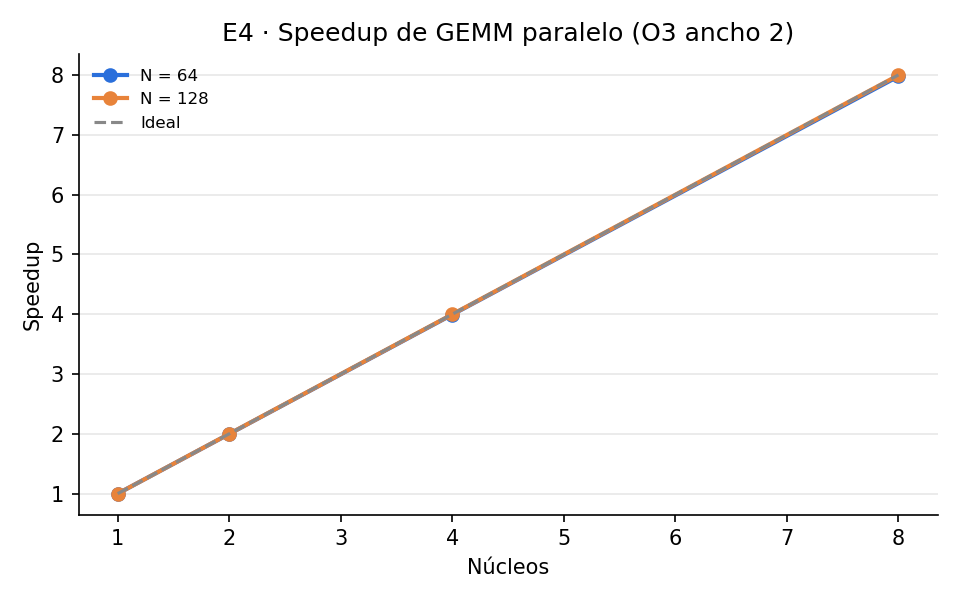
\includegraphics[width=\columnwidth]{fig/e4_speedup.png}
  \caption{\textit{Speedup} de GEMM paralelo frente al número de
    núcleos, con la recta ideal $S(p) = p$.}
  \label{fig:e4speedup}
\end{figure}

\begin{figure}[ht]
  \centering
  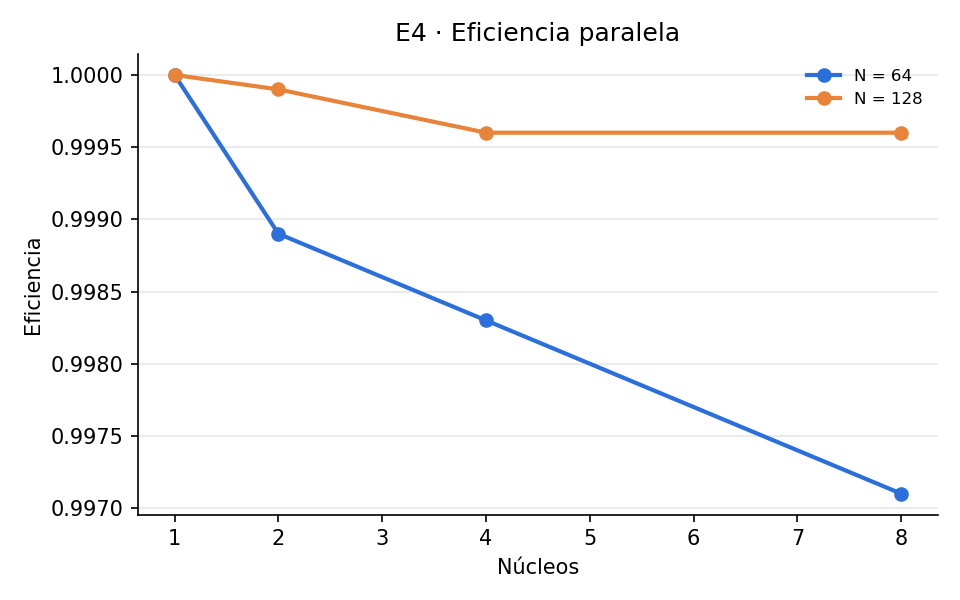
\includegraphics[width=\columnwidth]{fig/e4_efficiency.png}
  \caption{Eficiencia paralela $E(p) = S(p)/p$.}
  \label{fig:e4eff}
\end{figure}

\subsection{Análisis}

Que el \textit{speedup} sea casi ideal no es un accidente; se explica
por cuatro propiedades de la carga y de la medición:
\begin{enumerate}
  \item \textbf{Trabajo idéntico e independiente.} Cada hilo calcula
        $N/p$ filas completas de $C$ con exactamente el mismo número de
        operaciones, así que la carga está perfectamente balanceada. El
        total de instrucciones de la ROI apenas cambia con $p$: de
        \num{14779709} con un núcleo a \num{14780527} con ocho para
        $N=128$ ($+\SI{0{,}006}{\percent}$), diferencia que corresponde a
        las barreras.
  \item \textbf{Sin escrituras compartidas.} $A$ y $B$ solo se leen y
        cada hilo escribe filas distintas de $C$. Las líneas de $B$
        pueden estar copiadas en varias L1 a la vez en estado
        compartido sin generar invalidaciones, de modo que no hay
        tráfico de coherencia que serialice a los núcleos.
  \item \textbf{El conjunto de trabajo cabe en la L2.} Las tres
        matrices ocupan \SI{192}{KiB} con $N=128$, menos del
        \SI{10}{\percent} de la L2 de \SI{2}{MiB}, y quedaron en ella al
        inicializarlas. Por eso los fallos de L2 son despreciables (de
        3 a 24) y crecen exactamente en 3 por núcleo, lo que es consistente
        con fallos obligatorios sobre los datos privados de cada hilo
        y no con contención por la memoria principal.
  \item \textbf{La ROI solo mide la parte paralela.} La creación de
        los hilos, la inicialización y la verificación, que son las
        partes realmente seriales del programa, quedan fuera de la ROI
        por diseño de la medición.
\end{enumerate}

La Fig.~\ref{fig:e4l2} y los fallos de L1D de la Tabla~\ref{tab:e4}
muestran el único efecto de memoria visible. Con $N=64$ y un núcleo
los \SI{48}{KiB} de datos están en la L1D desde la inicialización y no
hay fallos; con $p$ núcleos, las L1 de los otros $p-1$ núcleos empiezan
vacías y cada una debe traer $B$ completa desde la L2, por lo que los
fallos de L1D crecen aproximadamente con $p$. Como los resuelve la L2
compartida con una latencia de unos 20 ciclos y su número es pequeño
frente al trabajo de cada núcleo, el costo es de a lo sumo el
\SI{0,3}{\percent}; es la causa de que la eficiencia con $N=64$ quede
ligeramente por debajo de la de $N=128$, donde cada núcleo tiene ocho
veces más trabajo para amortizar el mismo arranque en frío. Con
$N=128$ ocurre lo contrario: los \SI{192}{KiB} no caben en una sola L1D
y un núcleo sufre \num{32021} fallos de capacidad, pero repartidos entre
$p$ núcleos el total se mantiene entre \num{24000} y \num{28000}, porque
cada núcleo sigue recorriendo $B$ completa por cada fila.

\begin{figure}[ht]
  \centering
  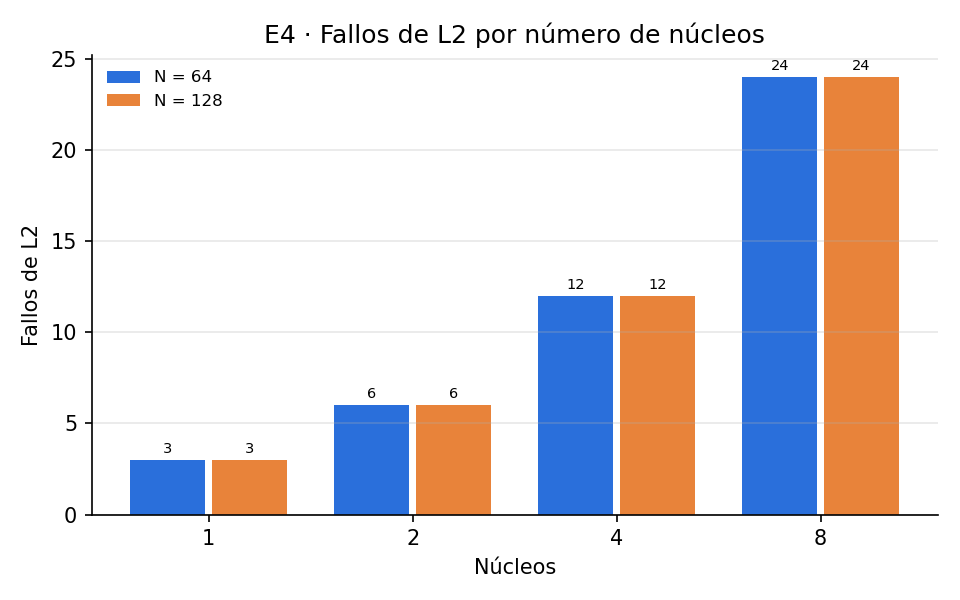
\includegraphics[width=\columnwidth]{fig/e4_l2_misses.png}
  \caption{Fallos de L2 en la ROI según el número de núcleos.}
  \label{fig:e4l2}
\end{figure}

\subsection{Medición del programa completo}

La ROI anterior responde cuánto escala el cálculo, pero deja fuera
justamente lo que Amdahl penaliza. Por eso se repitió E4 en un segundo
modo (\texttt{gemm\_omp N T full}, \texttt{MODE=full} en el script) en
el que la ROI cubre el programa real completo: la inicialización de
$A$, $B$ y $C$, que hace solo el hilo principal; la creación de los
hilos; el cálculo, y la espera de todos los hilos. Solo la verificación
queda fuera, porque no forma parte del trabajo útil.

\begin{table}[h]
\centering
\caption{E4 midiendo el programa completo (O3 de ancho 2).}
\label{tab:e4full}
\footnotesize
\setlength{\tabcolsep}{3pt}
\begin{tabular}{|c|c|r|c|c|c|}
\hline
$N$ & $p$ & \textbf{Ciclos} & $S(p)$ & $E(p)$ & $e(p)$ \\ \hline
64  & 1 & \num{2430635}  & $1{,}000$ & $1{,}000$ & ---        \\ \hline
64  & 2 & \num{1269371}  & $1{,}915$ & $0{,}957$ & $0{,}0445$ \\ \hline
64  & 4 & \num{685462}   & $3{,}546$ & $0{,}887$ & $0{,}0427$ \\ \hline
64  & 8 & \num{402391}   & $6{,}041$ & $0{,}755$ & $0{,}0463$ \\ \hline
128 & 1 & \num{19174455} & $1{,}000$ & $1{,}000$ & ---        \\ \hline
128 & 2 & \num{9744073}  & $1{,}968$ & $0{,}984$ & $0{,}0164$ \\ \hline
128 & 4 & \num{5024841}  & $3{,}816$ & $0{,}954$ & $0{,}0161$ \\ \hline
128 & 8 & \num{2674752}  & $7{,}169$ & $0{,}896$ & $0{,}0166$ \\ \hline
\end{tabular}
\end{table}

La Tabla~\ref{tab:e4full} y la Fig.~\ref{fig:e4full} muestran que ahora
la curva sí se separa de la ideal: con 8 núcleos el \textit{speedup} cae
a $7{,}17\times$ para $N=128$ y a $6{,}04\times$ para $N=64$, y la
eficiencia a $0{,}90$ y $0{,}76$. El ajuste de Amdahl da
$f = 0{,}0164$ para $N=128$ y $f = 0{,}0447$ para $N=64$, es decir, un
\textit{speedup} máximo de $1/f \approx 61\times$ y $22\times$.

Dos observaciones permiten atribuir esa pérdida a código serial y no a
contención entre núcleos:
\begin{itemize}
  \item \textbf{La métrica de Karp-Flatt es constante en $p$}
        ($0{,}0161$ a $0{,}0166$ con $N=128$). Si la pérdida viniera de
        sincronización, coherencia o competencia por la L2, $e(p)$
        crecería con el número de núcleos; que se mantenga constante es
        la firma de una fracción serial fija, exactamente el supuesto de
        la ley de Amdahl.
  \item \textbf{La fracción serial disminuye con $N$.} La inicialización
        recorre $N^2$ elementos, mientras que el cálculo hace $N^3$
        multiplicaciones y sumas; su peso relativo cae como $1/N$. Con un
        núcleo, la diferencia entre ambos modos es de \num{70852} ciclos
        (\SI{2,9}{\percent}) con $N=64$ y de \num{274942} ciclos
        (\SI{1,4}{\percent}) con $N=128$. El resto de $f$ lo aporta la
        creación de los hilos: el hilo principal ejecuta unas
        \num{2700} instrucciones adicionales por cada hilo que crea.
\end{itemize}
Los fallos de L2 suben de decenas a miles (de \num{2339} a \num{3179}
con $N=128$) porque la inicialización trae las matrices desde la
memoria principal por primera vez; son fallos obligatorios del
arranque, no un efecto del paralelismo.

\begin{figure}[ht]
  \centering
  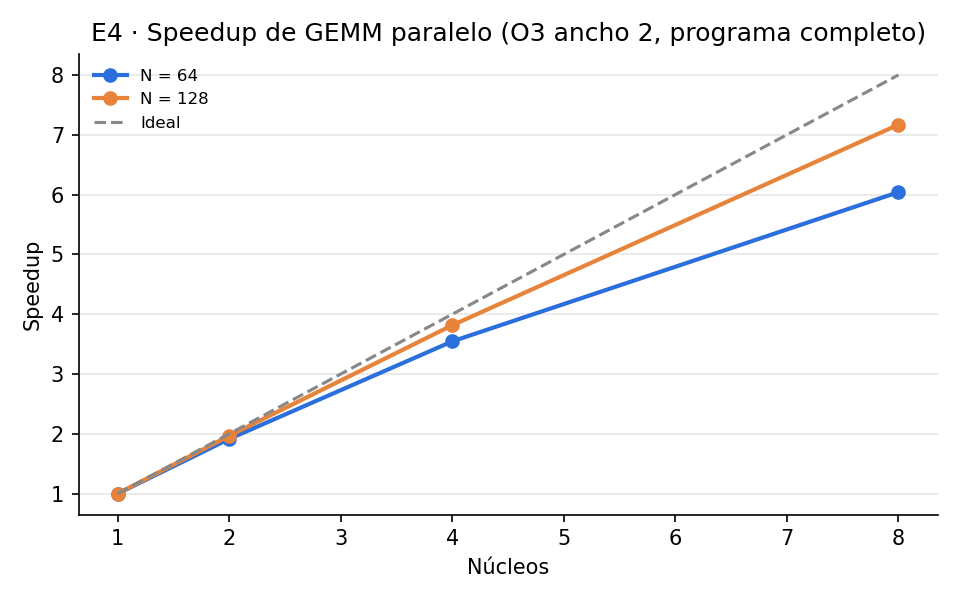
\includegraphics[width=\columnwidth]{fig/e4_full_speedup.png}
  \caption{\textit{Speedup} midiendo el programa completo
    (inicialización, creación de hilos, cálculo y espera).}
  \label{fig:e4full}
\end{figure}

\subsection{Respuesta a la pregunta guía}

La fracción serial que estima Amdahl depende de qué se mide. Para el
cálculo de GEMM por filas es de $8\times10^{-5}$ a $6\times10^{-4}$: el
núcleo de cómputo es, a efectos prácticos, completamente paralelo. Para
el programa completo es de \SI{1,6}{\percent} con $N=128$ y
\SI{4,5}{\percent} con $N=64$, y proviene de la inicialización serial y
de la creación de los hilos. Con $f = 0{,}0164$, 16 núcleos darían como
máximo $S = 1/(f + (1-f)/16) \approx 12{,}8\times$ y 32 núcleos
$\approx 21{,}2\times$: el rendimiento marginal de cada núcleo adicional
cae, lo que E6 debe considerar al repartir el presupuesto.

En la inferencia en el borde la inicialización ocurre una sola vez
(los pesos de la capa se cargan al arrancar) y GEMM se repite en cada
inferencia, de modo que el régimen relevante es el de la ROI de
cálculo. Ese régimen se mantiene mientras el conjunto de trabajo quepa
en la L2 compartida: con $N=1024$ las matrices ocupan \SI{12}{MiB}, no
caben en la L2 de \SI{2}{MiB}, y los núcleos competirían por el ancho
de banda de la memoria principal.

% =====================================================================
\section{E5: Coherencia de Memoria}
\label{sec:e5}

\pendiente{Integrante 4. MESI\_Two\_Level vs.\ MOESI\_CMP\_directory,
\texttt{false\_sharing} con y sin relleno y GEMM paralelo, 2 a 8 núcleos;
invalidaciones, mensajes y latencia de fallo. ¿Cuánto cuesta el falso
compartido? ¿Qué estado del protocolo genera el tráfico extra?}

% ===================== E6 =====================

\section{E6: Exploración Bajo Presupuesto}
\label{sec:e6}

\subsection{Metodología}

Todas las configuraciones ejecutan \texttt{gemm\_omp\_sve}: el mismo
reparto por filas de E4, pero con el kernel SVE de E3 dentro de cada
hilo, de modo que el programa aprovecha a la vez los núcleos y la
longitud vectorial por los que paga el modelo de costo. El ancho del O3
se fija como en E2 y la VL con el parámetro \texttt{sve\_vl\_se}. Se
reporta el tiempo de la ROI y el rendimiento en GFLOP/s ($2N^3/t$)
dividido por el costo. Cada configuración se agrega con una línea
(\texttt{CONFIGS="núcleos:ancho:VL[:protocolo]"}) y las corridas se
acumulan en \texttt{results/e6/}. Se evaluaron diez configuraciones con
$N=128$ y, para la sensibilidad al tamaño, tres de ellas con $N=256$
(\texttt{results/e6\_n256/}).

Cada configuración responde a un resultado previo: muchos núcleos
simples (E4 mostró escalabilidad casi lineal), VL largo con pocos
núcleos (E3 mostró que alargar VL rinde más por unidad de costo que
agregar núcleos), y variaciones del ancho con VL largo (E2 mostró que
el ancho no ayuda al código escalar, pero el kernel SVE tiene otro
perfil de dependencias).

\subsection{Resultados}

\begin{table}[!t]
\centering
\caption{Configuraciones de E6 con $N = 128$ (caches clásicas),
ordenadas por tiempo.}
\label{tab:e6}
\footnotesize
\setlength{\tabcolsep}{2pt}
\begin{tabular}{|c|c|c|c|c|c|c|}
\hline
\textbf{Núc.} & $W$ & \textbf{VL} & \textbf{Costo} &
\textbf{$t$ [ms]} & \textbf{GFLOP/s} & \textbf{GF/s/costo} \\ \hline
4  & 4 & 512  & 24 & $0{,}1032$ & $40{,}6$ & $1{,}693$ \\ \hline
2  & 8 & 1024 & 24 & $0{,}1082$ & $38{,}8$ & $1{,}616$ \\ \hline
2  & 4 & 1024 & 20 & $0{,}1082$ & $38{,}8$ & $1{,}938$ \\ \hline
16 & 2 & 128  & 32 & $0{,}1380$ & $30{,}4$ & $0{,}950$ \\ \hline
4  & 2 & 512  & 20 & $0{,}1403$ & $29{,}9$ & $1{,}495$ \\ \hline
2  & 2 & 1024 & 18 & $0{,}1491$ & $28{,}1$ & $1{,}563$ \\ \hline
1  & 4 & 1024 & 10 & $0{,}2155$ & $19{,}5$ & $1{,}946$ \\ \hline
1  & 8 & 1024 & 12 & $0{,}2156$ & $19{,}5$ & $1{,}621$ \\ \hline
8  & 2 & 128  & 16 & $0{,}2751$ & $15{,}2$ & $0{,}953$ \\ \hline
1  & 2 & 1024 & 9  & $0{,}2973$ & $14{,}1$ & $1{,}567$ \\ \hline
\end{tabular}
\end{table}

La Tabla~\ref{tab:e6} resume las diez configuraciones, todas con costo
menor o igual que 32.

\textbf{Muchos núcleos simples.} Las filas de 8 y 16 núcleos de ancho 2
y VL de 128 bits exploran la estrategia que sugiere E4: cada núcleo
cuesta 2 unidades. Duplicar los núcleos reduce el tiempo de
\SI{0,2751}{ms} a \SI{0,1380}{ms}, un factor de $1{,}994$: la
escalabilidad casi lineal de E4 se mantiene con el kernel vectorial y
con 16 hilos de solo 8 filas cada uno. Por eso el rendimiento por unidad
de costo es prácticamente el mismo ($0{,}953$ frente a $0{,}950$). El
kernel SVE también se nota frente a E4: con 8 núcleos de ancho 2, la
versión con VL de 128 bits termina en \num{550102} ciclos frente a
\num{2363489} de la escalar ($4{,}3\times$).

\textbf{Pocos núcleos con VL largo.} Con dos núcleos de ancho 4 y VL de
1024 bits (costo 20), GEMM termina en \SI{0,1082}{ms}: $1{,}27\times$ más rápido que con 16
núcleos simples, con un $37{,}5$\,\% menos de costo. Su rendimiento por unidad de costo
($1{,}94$) duplica el de los núcleos simples ($0{,}95$). Esto confirma
la predicción de E3: cada unidad de costo invertida en VL rinde más que
una invertida en núcleos de VL corto, porque un vector de 1024 bits
procesa 32 elementos con las mismas 12 instrucciones por iteración
del bucle que uno de 128 bits.

\textbf{Efecto del ancho.} A diferencia de E2, con el kernel SVE el
ancho sí importa, pero solo hasta 4. Con VL de 1024 bits, pasar de
ancho 2 a 4 reduce el tiempo un $27{,}5$\,\% con un núcleo
(\SI{0,2973}{ms} a \SI{0,2155}{ms}) y un $27{,}4$\,\% con dos
(\SI{0,1491}{ms} a \SI{0,1082}{ms}), mientras que pasar de 4 a 8 no
cambia el tiempo (diferencias menores que \SI{0,1}{\percent}). El IPC
por núcleo se mantiene en $2{,}09$ con ancho 4 y 8, de modo que a
partir de ancho 4 el límite son las dependencias del bucle (carga,
multiplicación-suma y almacenamiento de la misma fila de $C$) y no el
número de instrucciones que el núcleo puede emitir. El ancho 8 solo
agrega costo.

\textbf{Núcleos con VL largo.} Con ancho 4 y VL de 1024 bits, pasar de
uno a dos núcleos reduce el tiempo $1{,}99\times$: el reparto por filas
sigue escalando casi linealmente con el kernel vectorial.

\subsection{Configuración recomendada}

\begin{itemize}
  \item \textbf{Menor tiempo:} 4 núcleos, ancho 4 y VL de 512 bits
    (costo 24), con \SI{0,1032}{ms}.
  \item \textbf{Mejor rendimiento por costo:} 1 núcleo, ancho 4 y VL de
    1024 bits (costo 10) y 2 núcleos con la misma configuración
    (costo 20) empatan ($1{,}946$ y $1{,}938$ GFLOP/s por unidad).
\end{itemize}

Se recomienda \textbf{2 núcleos, ancho 4 y VL de 1024 bits (costo 20)}.
Queda a un $4{,}9$\,\% de la configuración más rápida con un
$17$\,\% menos de costo, comparte el mejor rendimiento por unidad de
costo y deja 12 unidades del presupuesto sin usar. Si el único criterio
es el tiempo de GEMM con $N=128$, como plantea la pregunta del
proyecto, la respuesta estricta es 4 núcleos, ancho 4 y VL de 512 bits.

\subsection{Análisis de sensibilidad}

\textbf{Presupuesto de 16.} Con costo menor o igual que 16 quedan cuatro
de las configuraciones evaluadas. La mejor es 1 núcleo, ancho 4 y VL de
1024 bits (costo 10, \SI{0,2155}{ms}), que es $1{,}28\times$ más rápida
que 8 núcleos simples (costo 16, \SI{0,2751}{ms}) y usa 6 unidades
menos. Con un presupuesto ajustado, la conclusión se mantiene: conviene
gastar en VL y en ancho 4 antes que en núcleos. Combinaciones de costo
intermedio como 2 núcleos, ancho 4 y VL de 512 bits (costo 12) no se
evaluaron y podrían mejorar este resultado.

\begin{table}[!t]
\centering
\caption{Sensibilidad al tamaño: tres configuraciones con $N = 256$.}
\label{tab:e6_n256}
\footnotesize
\setlength{\tabcolsep}{2pt}
\begin{tabular}{|c|c|c|c|c|c|c|}
\hline
\textbf{Núc.} & $W$ & \textbf{VL} & \textbf{Costo} &
\textbf{$t$ [ms]} & \textbf{GFLOP/s} & \textbf{Fallos L1D} \\ \hline
16 & 2 & 128  & 32 & $1{,}1301$ & $29{,}7$ & $33{,}0$\,\% \\ \hline
2  & 4 & 1024 & 20 & $1{,}6109$ & $20{,}8$ & $26{,}6$\,\% \\ \hline
8  & 2 & 128  & 16 & $2{,}1614$ & $15{,}5$ & $30{,}8$\,\% \\ \hline
\end{tabular}
\end{table}

\textbf{Tamaño de la matriz.} Simular $N=1024$ requiere 512 veces el
trabajo de $N=128$ y no fue viable en el tiempo del proyecto, por lo que
se midió $N=256$ (Tabla~\ref{tab:e6_n256}) para identificar la
tendencia. El orden se invierte: con $N=256$, los 16 núcleos simples
son $1{,}43\times$ más rápidos que la configuración recomendada. Los
núcleos simples mantienen su rendimiento ($30{,}4$ a $29{,}7$ GFLOP/s
con 16 núcleos y $15{,}2$ a $15{,}5$ con 8), mientras que la de 2 núcleos
con VL de 1024 bits cae de $38{,}8$ a $20{,}8$ GFLOP/s ($-46$\,\%): su
tiempo crece $14{,}9\times$ cuando el trabajo crece $8\times$.

La causa es la memoria. Con $N=256$ las tres matrices ocupan
\SI{768}{KiB}, doce veces la L1D, y la tasa de fallos de L1D pasa de
cerca del 3\,\% al 27--33\,\% en todas las configuraciones. Los fallos de
L2 siguen siendo despreciables (8 a 50), así que los datos se sirven
desde la L2 de \SI{2}{MiB}. Con 16 núcleos hay 16 L1D privadas y 16
flujos de fallos que se atienden en paralelo; con 2 núcleos, cada fallo
detiene a una fracción mayor de la máquina y cada acceso de 1024 bits
abarca dos líneas, como se vio en E3. El IPC por núcleo de la
configuración recomendada baja de $2{,}08$ a $1{,}05$. Aun así sigue
teniendo el mejor rendimiento por unidad de costo ($1{,}04$ frente a
$0{,}93$ y $0{,}97$), aunque la ventaja se reduce de $2{,}0\times$ a
$1{,}1\times$.

Con $N=1024$ las matrices ocupan \SI{12}{MiB} y superan también la
L2, de modo que el acceso a DRAM dominaría. Por extrapolación de la
tendencia medida, las configuraciones con pocos núcleos y VL largo
perderían aún más frente a las de muchos núcleos, y la recomendación se
desplazaría hacia más núcleos. Para ese tamaño, más que cambiar la
configuración, convendría reorganizar el algoritmo con bloqueo por
caché \cite{goto2008} para que cada bloque quepa en la L1D, lo que
devolvería a GEMM al régimen de $N=128$ donde el VL largo es la mejor
inversión.

% =====================================================================
\section{Conclusiones}
\label{sec:conclusiones}

\pendiente{respuesta a la pregunta del proyecto: configuración
recomendada, su costo y tiempo, y las alternativas descartadas con su
justificación.}

\pendiente{enlace al video de conclusiones en YouTube (no listado).}

\printbibliography

\end{document}
